\documentclass{article}
\usepackage[T1]{fontenc}
\usepackage{lmodern}
\usepackage{graphicx}
\usepackage{amsmath,amssymb}
\usepackage[a4paper,margin=2cm]{geometry}
\usepackage[absolute,overlay]{textpos}
\setlength{\TPHorizModule}{1mm}
\setlength{\TPVertModule}{1mm}
\usepackage[indonesian]{babel}
\usepackage{hyperref}
\setlength{\emergencystretch}{2em}
% unit: Halaman 4

\begin{document}

% === Halaman 4 (llm) ===

\vspace{219.78mm}

\begin{center}
\Huge Diagram Blok Kriptografi Modern
\end{center}

\vspace{10mm}

% deskripsi: Diagram blok kriptografi modern yang menunjukkan hubungan hierarkis antara protokol jaringan aman (Secure Network Protocols), tujuan keamanan (Confidentiality, Data Integrity, Authentication, Non-Repudiation), mekanisme implementasi (Encryption, MACs/MICs, Challenge Responses, Digital Signatures), metode kriptografi (Symmetric Key Cryptography, Message Digest, Public Key Cryptography), dan komponen dasar (Block Cipher, Stream Cipher, Hash Function, Pseudo Random, Random Source, Elliptic Curve, DH RSA).
% bbox normalisasi: [0.1800, 0.1700, 0.8200, 0.9100]
\begin{textblock*}{134.40mm}(37.80mm,50.49mm)
\noindent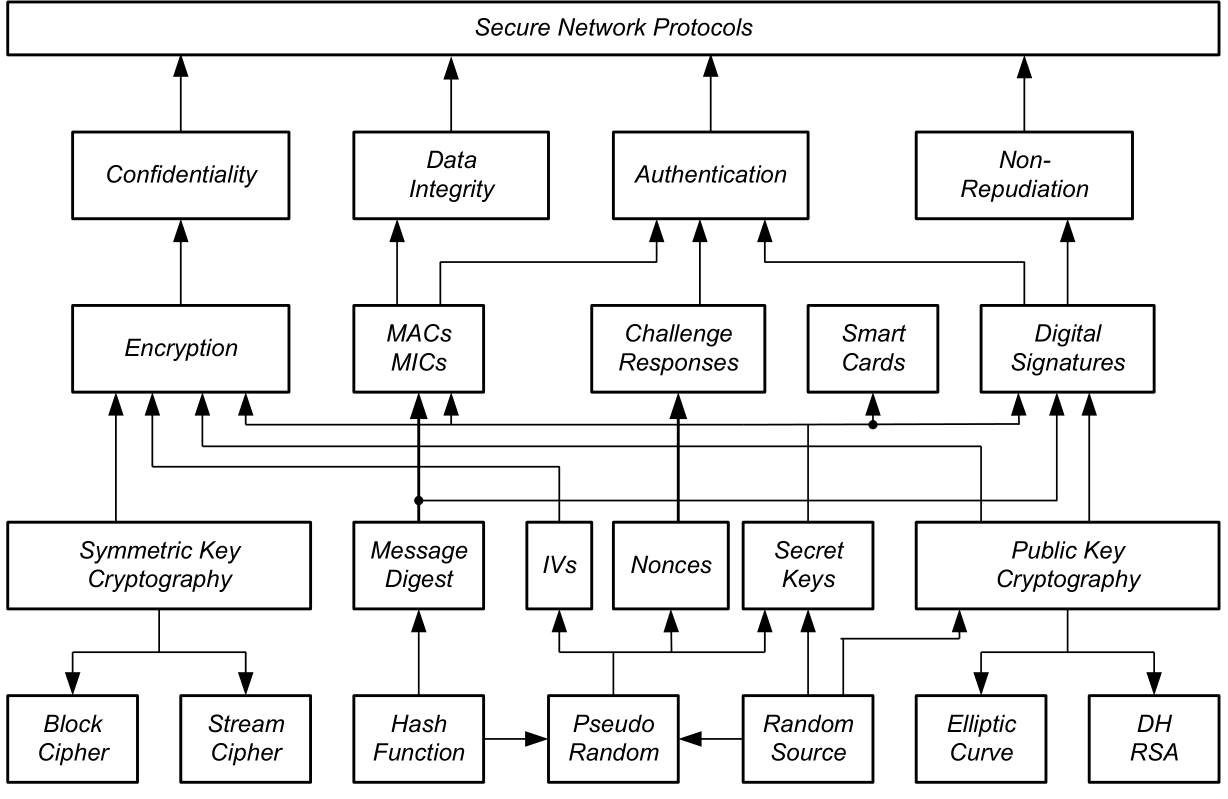
\includegraphics[width=134.40mm,height=219.78mm]{../../images/llm/page_004_img_01.png}%
\end{textblock*}

\end{document}
